\documentclass[citeauthoryear]{llncs} %
\usepackage[utf8]{inputenc}
\usepackage{graphicx}
\bibliographystyle{splncs}

\begin{document}

\title{Implementação de um robô reativo para o simulador Ciber-Rato}
\author{Tiago Babo e Hélder Moreira}

\institute{Faculdade de Engenharia da Universidade do Porto}

\maketitle

\begin{abstract}
This paper describes a reactive robotic agent for the Ciber-Rato platform. The algorithm used by the robot, based on the behaviour “follow wall” - when possible - doesn't save previous information and can finish some types of mazes easily.
\end{abstract}

\section{Introdução}
O simulador Ciber-Rato (\cite{microrato}) surgiu no âmbito de um concurso de robótica móvel organizado pela Universidade de Aveiro. O objetivo das equipas é construir um algoritmo de controlo que comanda um robô virtual, com a finalidade de resolver um labirinto. 

Para resolver o labirinto, o robô deve encontrar um objeto em específico (representado por um queijo, normalmente).

Este artigo descreve uma possível implementação de um robô reativo que consegue resolver um determinado número de configurações de obstáculos e labirintos, recorrendo a um algoritmo que tenta contornar paredes. 

\section{Robô Virtual}

O robô virtual é constituído por uma forma circular, equipado com sensores, atuadores e botões de comando. 

\subsection{Sensores}
Para o desenvolvimento do algoritmo foi considerado que o robô possui: três sensores de obstáculos, um sensor de farol, que lhe indica a direção da zona de chegada, um sensor de colisões binário e um sensor que lhe diz se está na área do objetivo. 

Os sensores têm diferentes resoluções, ruído associado e pode haver alguma latência na sua leitura.

\subsection{Atuadores}

O robô possui dois motores, representando duas rodas, que permitem efetuar translações ou rotações da sua posição. É possível especificar a força aplicada a cada roda. 

Quando o robô atinge o objetivo final deve sinalizar que lá chegou, através dos \emph{leds} que possui. 

\subsection{Botões de Comando}
Os botões de comando, \emph{Start} e \emph{Stop}, permitem ao simulador controlar o decorrer da competição.

\section{Simulador}

O simulador Ciber-Rato é responsável por:
\begin{enumerate} 
\item Implementar o labirinto virtual 
\item Implementar o corpo virtual do robô
\item Coordenar o movimento dos robôs no labirinto em articulação com o agente
\item Desempenhar o papel de juiz virtual da prova:
\begin{enumerate} 
\item Controla o tempo da prova
\item Aplica as penalizações (choque com obstáculos, por exemplo)
\item Calcula as pontuações
\end{enumerate}
\end{enumerate}

O cenário da competição é delineado por uma área retangular, delimitada, composta por obstáculos, uma área objetivo e várias posições onde os robôs podem começar. Em relação aos obstáculos, estes podem ter alturas diferentes, influenciando a leitura do sensor de farol do robô. Se o obstáculo ultrapassar uma certa altura, o robô deixa de conseguir receber a informação proveniente do sensor. 

\section{Algoritmo usado}

O algoritmo usado adota uma estratégia puramente reativa. Segundo Ronald C. Arkin, esta metedologia permite uma resposta rápida e flexível do sistema. É caracterizada por uma estrutura baseada em blocos de comportamento com diferentes prioridades e por não guardar qualquer informação sobre o estado do mundo e reagindo apenas às informações do presente. (\cite{arkin})

Desta forma, a estratégia adotada segue as seguintes prioridades:

\begin{enumerate}
\item Evitar obstáculo
\item Alinhar-se com a direção do objetivo
\item Andar em frente
\end{enumerate}

Para evitar um obstáculo, é usado um algoritmo de contorno de paredes, mantendo esta estratégia até que consiga ver o farol e esteja enquadrado com ele, considerando uma amplitude de 20º. O robô desloca-se sempre no sentido dos ponteiros do relógio.   

\begin{figure}[htb]
\begin{center}
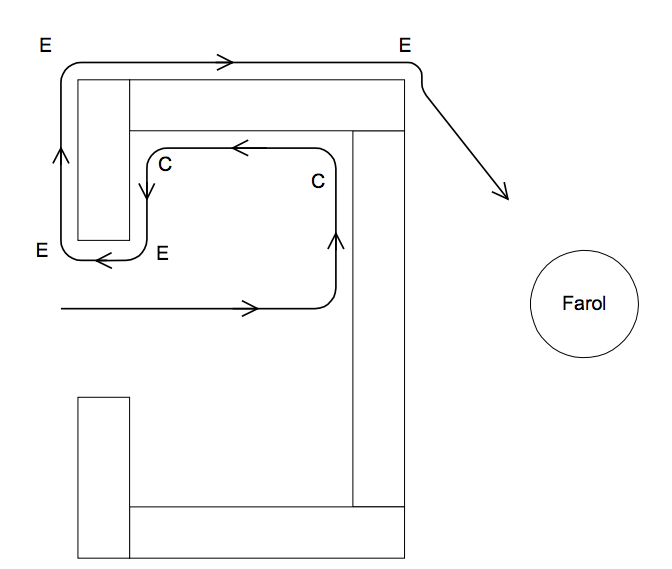
\includegraphics[scale=0.30]{fig1.png}
\caption{Exemplo de um obstáculo contornável}
\end{center}
\end{figure}

Este método consegue resolver diferentes tipos de configurações. A figura 1 representa um obstáculo complexo que pode ser evitado com o algoritmo desenvolvido. O robô começa por se deslocar em frente. Quando verifica que há uma parede à sua frente, roda no sentido contrário ao dos ponteiros do relógio até se encontrar com a parede do seu lado direito (cerca de 90º). Depois, continua em frente. Nos pontos C (e de forma generalizada, em todos os cantos) o mecanismo é  semelhante ao descrito anteriormente. No caso dos pontos E, que representam esquinas, o robô posiciona-se de forma a afastar-se o suficiente para conseguir rodar no sentido dos ponteiros do relógio e seguir em frente sem bater na esquina. Aquando a rotação na esquina, é verificado se o robô consegue receber informação sobre a direção do objetivo e, em caso afirmativo, se a direção de este se encontrar num intervalo de 20º. Caso tal se verifique, o contorno da parede é abortado e o robô segue em direção ao objetivo.

No entanto, este algoritmo não consegue resolver um tipo específico de labirintos. Como não é guardada nenhuma informação sobre o contorno da parede - mesmo o próprio facto de a estarmos a contornar - torna-se difícil evitar que o robô entre em ciclos, a não ser que consiga obter informação do objetivo passível de abortar o contorno e que não o faça recomeçar o contorno da mesma parede.  

\begin{figure}[htb]
\begin{center}
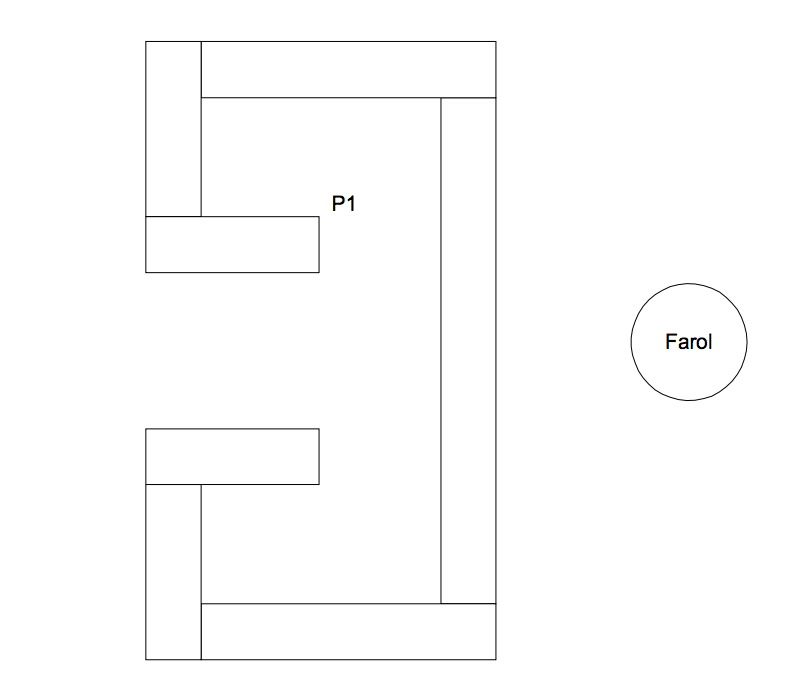
\includegraphics[scale=0.20]{fig2.png}
\caption{Exemplo de um obstáculo que conduz a um ciclo}
\end{center}
\end{figure}


Tal como se pode ver na figura 2, em que há uma parede de altura inferior à mínima para o robô não obter informação do objetivo, o robô desloca-se na sua direção. Ao verificar que se encontra em frente a uma parede, começa a contorna-la. Ao dobrar a esquina P1, e segundo o método descrito anteriormente, o robô vai obter informação que o faz abortar o contorno da parede. Ao deslocar-se no sentido do objetivo, acaba por ir novamente em direção à parede, reiniciando o processo. Desta forma, entra em ciclo infinito. No entanto, se esta parede atingisse a altura mínima, o robô não obteria informação que o fizesse abortar o contorno, e, tal como na figura 1, atingiria o objetivo.   

\begin{figure}[htb]
\begin{center}
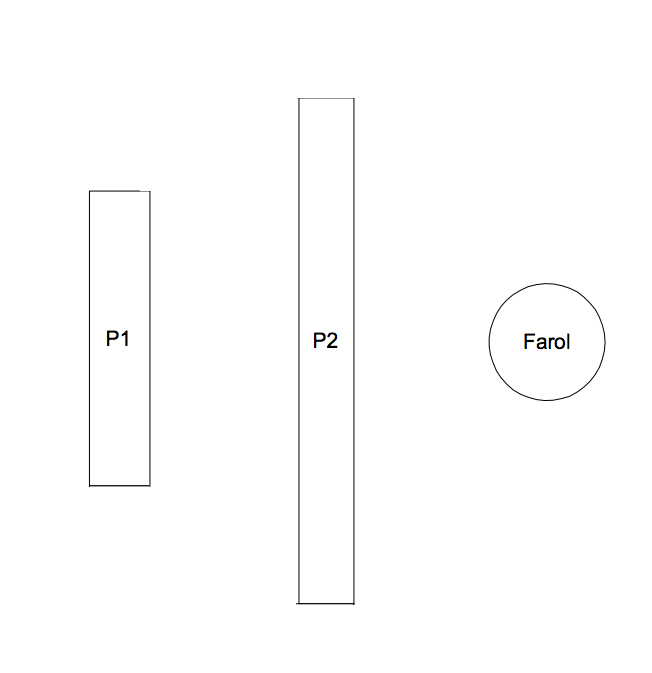
\includegraphics[scale=0.20]{fig3.png}
\caption{Exemplo de um obstáculo que conduz a um ciclo}
\end{center}
\end{figure}

A figura 3 exemplifica outro caso em que o algoritmo desenvolvido entra em ciclo. Sejam consideras duas paredes paralelas, de altura mínima para o robô não receber informação do objetivo quando se encontra atrás das mesmas. Desta forma, quando se aproxima de P1, começa a contornar a parede. No entanto, como em nenhum momento do contorno o robô obtém informação do objetivo, acaba por entrar em ciclo. Mais uma vez, como não é guardada informação nenhuma, é impossível, com esta abordagem, evitar este tipo de configurações.

Os problemas descritos na figura 2 e na figura 3 podiam ser evitados caso se implementasse um algoritmo mais complexo, e que acabaria por tornar o robô menos reativo. Seguindo o exemplo do EnCuRRalado (\cite{encur}) e mantendo o número de cantos e o número de esquinas no contorno da parede, seria possível evitar os problemas descritos pelo algoritmo implementado.

\section{Conclusões}

A solução apresentada baseia-se numa abordagem puramente reativa e num algoritmo de contorno de parede simples. Apesar de resolver uma inúmera quantidade de labirintos, há determinados cenários conhecidos em que falha na sua tarefa. De forma genérica, quando no contorno da parede não se obtém a informação necessária para o terminar, o robô acaba por entrar em ciclo.

A evolução natural deste algoritmo seria, então, alterar a abordagem puramente reativa e guardar informação que permitisse detetar e tentar mitigar os problemas conhecidos.

\begingroup
\renewcommand\refname{Referências}
\begin{thebibliography}{}

\bibitem[Micro-Rato 2011]{microrato}
Micro-Rato, Departamento de Eletrónica e Telecomunicações, Universidade de Aveiro, 2011, "CiberRato 2011 - Rules and Technical Specifications" Acedido a 3 de Novembro 2012. http://microrato.ua.pt
\bibitem[1995]{arkin}
Arkin, R. (1995). Reactive robotic systems. The handbook of brain theory and neural networks, (404), 1–12
\bibitem[Luís et al.  2002]{encur}
Luís, P., Martins, B., Almeida, P., e Silva, V. (1999). Detecção de configurações de obstáculos perigosas: aplicação no robô EnCuRRalado. 
\end{thebibliography}
\endgroup
\end{document}